\section{2022 Geometry \& Topology}

\subsection{Exam}

\begin{exercise}
\label{geometry:2022:1}
The topological space $X$ is obtained by gluing two tetrahedra as illustrated. The resulting complex has 2 tetrahedra, 4 triangles, 2 edges and 1 vertex. Show that $X$ cannot have the homotopy type of a compact manifold without boundary.
\end{exercise}

\begin{center}
  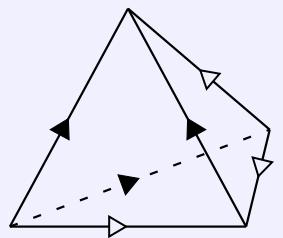
\includegraphics[width=0.45\textwidth]{images/geometry/1dcad16590d701da49d529ca0c5c5ca15cc5c79f8009620e6d8d236d0acc0986.jpg}
  \\
  \captionof{figure}{Two tetrahedra being glued (I)}
\end{center}
\hfill
\begin{center}
  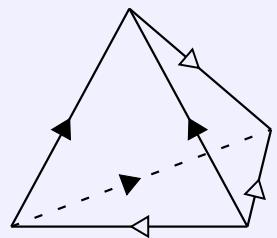
\includegraphics[width=0.45\textwidth]{images/geometry/e4a7113eed10b3cd0e2d8962fbb743b0a91bc5165d0c09d169d74b273f07abfa.jpg}
  \\
  \captionof{figure}{Two tetrahedra being glued (II)}
\end{center}

\begin{solution}
\textbf{Prerequisites / Core Concepts:}
\begin{itemize}
    \item \textbf{Euler Characteristic ($\chi$):} For a topological space $X$, $\chi(X)$ is defined as the alternating sum of its Betti numbers $b_k = \operatorname{rank} H_k(X)$:
    \begin{equation*}
        \chi(X) = \sum_{k=0}^{\dim X} (-1)^k b_k(X) = b_0 - b_1 + b_2 - \dots
    \end{equation*}

    \item \textbf{Formula for CW Complexes:} For an $n$-dimensional CW complex, let $c_k$ be the number of $k$-cells. The formula is:
    \begin{equation*}
        \chi(X) = \sum_{k=0}^{n} (-1)^k c_k = c_0 - c_1 + c_2 - \dots + (-1)^n c_n
    \end{equation*}
    \sidenote{Cell Addition Logic: Adding a $k$-cell $\sigma^k$ to a $(k-1)$-skeleton $X_{k-1}$ changes the Euler characteristic by $\chi(X_{k-1} \cup \sigma^k) = \chi(X_{k-1}) + (-1)^k$. In terms of homology, this either creates a new $k$-cycle ($b_k \to b_k + 1$) or kills a $(k-1)$-cycle ($b_{k-1} \to b_{k-1} - 1$). In both cases, $\Delta \sum (-1)^i b_i = (-1)^k$.}

    \item \textbf{Cellular Chain Complex Argument:} 
    The rank-nullity theorem applied to the boundary operators $\partial_k$ in the cellular chain complex $C_k(X)$ ensures that $\sum (-1)^k \operatorname{rank}(C_k) = \sum (-1)^k \operatorname{rank}(H_k)$. This identity allows us to compute the Euler characteristic by simply counting the cells of each dimension.

    \item \textbf{Manifold Condition and Link:}\footnote{The link $\operatorname{Lk}(v, K)$ of a vertex $v$ in a simplicial complex $K$ is the set of all simplices $\tau$ such that $v \cup \tau$ is a simplex in $K$ but $v \notin \tau$. For a 3-manifold, the neighborhood of every point is a 3-ball, and the boundary of this ball (the link) is a 2-sphere.} For a 3-dimensional simplicial complex to be a manifold without boundary, the link of every vertex must be homeomorphic to a 2-sphere $S^2$.
    
    \item \textbf{Poincaré Duality Constraint:}\footnote{Poincaré Duality states $H_i(M; \mathbb{Z}) \cong H^{n-i}(M; \mathbb{Z})$ for oriented closed manifolds. Thus $b_i = b_{n-i}$. If $n$ is odd, the terms in $\chi = \sum_{i=0}^n (-1)^i b_i$ cancel in pairs: $(-1)^i b_i + (-1)^{n-i} b_{n-i} = (-1)^i b_i + (-1)^{n-i} b_i = 0$ since $i$ and $n-i$ have opposite parity.} For a closed, connected, oriented $n$-manifold $M$, the Euler characteristic must satisfy $\chi(M) = 0$ if $n$ is odd.
\end{itemize}

\textbf{Steps:}
\begin{enumerate}
    \item \textbf{Calculate the Euler Characteristic of $X$:} 
    The space $X$ is composed of $V = 1$ vertex, $E = 2$ edges, $F = 4$ triangles, and $T = 2$ tetrahedra. Using the cell count formula:
    \[ \chi(X) = V - E + F - T = 1 - 2 + 4 - 2 = 1. \]

    \item \textbf{Global Topological Obstruction:} 
    If $X$ were a compact 3-manifold without boundary, Poincaré Duality would imply $\chi(X) = 0$. However, we calculated $\chi(X) = 1$. Since $1 \neq 0$, $X$ cannot be a closed 3-manifold.

    \item \textbf{Local Analysis via the Link:}
    To verify the non-manifold nature locally, we examine the link $\operatorname{Lk}(v)$ of the single vertex $v$.
    \begin{itemize}
        \item The number of vertices, edges, and faces in $\operatorname{Lk}(v)$ corresponds to the number of edges, triangles, and tetrahedra incident to $v$ in $X$.
        \item Given $E_{inc} = 2$, $F_{inc} = 4$, and $T_{inc} = 2$, the link has $V_{\operatorname{Lk}} = 2$, $E_{\operatorname{Lk}} = 4$, and $F_{\operatorname{Lk}} = 2$.
        \item Calculating the Euler characteristic of the link:
        \[ \chi(\operatorname{Lk}(v)) = V_{\operatorname{Lk}} - E_{\operatorname{Lk}} + F_{\operatorname{Lk}} = 2 - 4 + 2 = 0. \]
        \sidenote{Link Calculation: $\chi(\operatorname{Lk}(v)) = 2 - 2\chi(X) = 2 - 2(1) = 0$. For a 3-manifold, we must have $\chi(\operatorname{Lk}(v)) = \chi(S^2) = 2$.}
        \item A 2D complex with $\chi = 0$ is a torus or a Klein bottle, not a 2-sphere.
    \end{itemize}
    \item \textbf{Conclusion:} $X$ fails both the global parity requirement for 3-manifolds and the local link condition. Thus, $X$ is a singular space (a pseudo-manifold) that cannot have the homotopy type of a compact 3-manifold without boundary.
\end{enumerate}

\textbf{Intuition:}
In a manifold, every point is surrounded by a "normal" neighborhood. In this construction, the way the tetrahedra are pinched together at a single vertex creates a singularity. The Euler characteristic captures this imbalance: a value of 1 instead of 0 signals that the space is "topologically asymmetric," possessing a structure that doesn't "smooth out" like a manifold.
\end{solution}

\begin{exercise}
\label{geometry:2022:2}
Suppose $(M, h)$ is a closed Riemannian manifold with $\sec(h) \leq -1$. Suppose $\Sigma$ is a closed minimal surface with genus $g$ in $(M, h)$. Show that $\operatorname{Area}(\Sigma) \leq 4\pi(g - 1)$.
\end{exercise}

\begin{solution}
\textbf{Prerequisites:}
\begin{itemize}
    \item \textbf{Sectional Curvature ($\sec$):} A measure of the curvature of a 2-plane in the tangent space. $\sec(P) \leq -1$ implies the manifold is "globally hyperbolic" or negatively curved.
    \item \textbf{Minimal Surface:}\footnote{A minimal surface $\Sigma \subset M$ is a critical point of the area functional. This is equivalent to the mean curvature $H = \operatorname{tr}(h)$ vanishing identically, where $h$ is the second fundamental form.} A surface where the mean curvature $H = \kappa_1 + \kappa_2$ is zero at every point.
    \item \textbf{Gauss Equation:} $K_\Sigma = \sec_M(T\Sigma) + \det(h)$. This relates the intrinsic Gaussian curvature of the surface to the ambient sectional curvature and the extrinsic second fundamental form.
    \item \textbf{Gauss-Bonnet Theorem:} For a closed surface $\Sigma$, $\int_\Sigma K_\Sigma \, dA = 2\pi \chi(\Sigma) = 4\pi(1 - g)$.
    \sidenote{Betti number derivation: For a closed oriented surface of genus $g$, $b_0=1, b_2=1$, and $b_1=2g$ (representing $g$ pairs of longitude and meridian loops). Thus $\chi = b_0 - b_1 + b_2 = 1 - 2g + 1 = 2 - 2g$.}
\end{itemize}

\textbf{Steps:}
\begin{enumerate}
    \item \textbf{Calculate Intrinsic Curvature:} 
    Let $\kappa_1, \kappa_2$ be the principal curvatures of $\Sigma \subset M$. The Gauss equation gives:
    \[ K_\Sigma = \sec_M(T\Sigma) + \kappa_1 \kappa_2. \]
    Since $\Sigma$ is minimal, $H = \kappa_1 + \kappa_2 = 0 \implies \kappa_2 = -\kappa_1$.
    \item \textbf{Apply Curvature Bounds:} 
    Substituting the minimality condition:
    \[ K_\Sigma = \sec_M(T\Sigma) - \kappa_1^2. \]
    \sidenote{Curvature Bound: Since $\sec_M \leq -1$ and $\kappa_1^2 \geq 0$, we have $K_\Sigma \leq -1 - \kappa_1^2 \leq -1$.}
    This inequality shows that a minimal surface in a negatively curved space must be at least as negatively curved as the ambient space.
    \item \textbf{Integrate over the Surface:} 
    Integrating the inequality $K_\Sigma \leq -1$ over $\Sigma$:
    \[ \int_\Sigma K_\Sigma \, dA \leq \int_\Sigma (-1) \, dA = -\operatorname{Area}(\Sigma). \]
    Applying the Gauss-Bonnet theorem to the left-hand side:
    \[ 2\pi(2 - 2g) \leq -\operatorname{Area}(\Sigma). \]
    
    \item \textbf{Conclusion:} 
    Multiplying by $-1$ and rearranging:
    \[ \operatorname{Area}(\Sigma) \leq -2\pi(2 - 2g) = 4\pi(g - 1). \]
    Note that this also implies $g \geq 1$, as a minimal surface in $\sec \leq -1$ cannot be a sphere ($g=0$).
\end{enumerate}

\textbf{Intuition:}
The "tightness" of a minimal surface in a space that is flaring out (negative curvature) forces the surface to have a negative Gaussian curvature. This negative curvature is proportional to the surface area. The topological genus $g$ provides the "budget" for this curvature; higher genus allows for more area, but the $-1$ curvature bound puts a strict limit on that area for any given $g$.
\end{solution}

\begin{exercise}
\label{geometry:2022:3}
Show that $\mathsf{SP}^{n}(\mathbb{CP}^{1})$ is homeomorphic to $\mathbb{CP}^{n}$.
\end{exercise}

\begin{solution}
\textbf{Prerequisites:}
\begin{itemize}
    \item \textbf{Symmetric Product ($\mathsf{SP}^n$):} The space of unordered multisets of $n$ points in $X$, defined as the quotient $(X \times \dots \times X) / S_n$.
    \item \textbf{Projective Line ($\mathbb{CP}^1$):} Points $[u : v]$ representing lines in $\mathbb{C}^2$, topologically a sphere (the Riemann sphere).
    \item \textbf{Fundamental Theorem of Algebra:}\footnote{The Fundamental Theorem of Algebra states that every non-constant homogeneous polynomial $P(z, w)$ of degree $n$ over $\mathbb{C}$ factors uniquely into $n$ linear factors $L_i(z, w) = v_i z - u_i w$. These factors correspond to the roots $[u_i : v_i] \in \mathbb{CP}^1$.} Relates roots to coefficients of polynomials.
\end{itemize}

\textbf{Steps:}
\begin{enumerate}
    \item \textbf{Construct the Root-to-Coefficient Map:} 
    An element in $\mathsf{SP}^n(\mathbb{CP}^1)$ is a set of $n$ points $\{[u_i : v_i]\}_{i=1}^n$. We define a map $\Phi: \mathsf{SP}^n(\mathbb{CP}^1) \to \mathbb{CP}^n$ by forming the product:
    \[ P(z, w) = \prod_{i=1}^n (v_i z - u_i w) = a_0 z^n + a_1 z^{n-1} w + \dots + a_k z^{n-k} w^k + \dots + a_n w^n. \]
    The coefficients $a_k$ are determined by the expansion of the product:
    \[ a_k = (-1)^k \sum_{|S|=k} \left( \prod_{i \in S} u_i \prod_{j \notin S} v_j \right) \]
    where $S$ ranges over all $k$-element subsets of $\{1, \dots, n\}$.
    \sidenote{Explicit Form: For $n=2$, $a_0 = v_1 v_2$, $a_1 = -(u_1 v_2 + u_2 v_1)$, and $a_2 = u_1 u_2$. In general, $a_k = (-1)^k \sigma_k(u, v)$ where $\sigma_k$ is the multi-homogeneous symmetric polynomial.}
    \sidenote{Elementary Symmetric Polynomials: On the chart $v_i \neq 0$, let $x_i = u_i/v_i$. Then $a_k = (\prod v_i) (-1)^k e_k(x_1, \dots, x_n)$, where $e_k$ is the $k$-th elementary symmetric polynomial.}

    \item \textbf{Verification of Well-definedness:}
    \begin{itemize}
        \item \textbf{Permutation Invariance:} The product $\prod (v_i z - u_i w)$ is commutative, so the coefficients $a_k$ are invariant under permutations of the indices $i$.
        \item \textbf{Scaling Invariance:} If a point $[u_j : v_j]$ is scaled by $\lambda$, the vector $(a_0, \dots, a_n)$ is scaled by $\lambda$. This preserves the point in $\mathbb{CP}^n$.
    \end{itemize}

    \item \textbf{Bijectivity:}
    \begin{itemize}
        \item \textbf{Injectivity:} By the unique factorization of polynomials, the coefficients $[a_0 : \dots : a_n]$ uniquely determine the roots $\{[u_i : v_i]\}$ as an unordered set.
        \item \textbf{Surjectivity:} Any point in $\mathbb{CP}^n$ defines a non-zero degree $n$ polynomial, which always factors into $n$ roots by the Fundamental Theorem of Algebra.
    \end{itemize}

    \item \textbf{Homeomorphism:}
    The map $\Phi$ is continuous as the coefficients are polynomial functions of the coordinates. Since $\mathsf{SP}^n(\mathbb{CP}^1)$ is compact and $\mathbb{CP}^n$ is Hausdorff, the continuous bijection $\Phi$ is a homeomorphism.
\end{enumerate}

\textbf{Intuition:}
The space of "unlabeled roots" is identical to the space of "polynomial coefficients." In the complex world, every collection of $n$ points on a sphere can be fused into a single polynomial, and every polynomial can be decomposed into exactly $n$ points. This map perfectly preserves the topology of how these collections can move and merge.
\end{solution}

\begin{exercise}
\label{geometry:2022:4}
Show that if a complete noncompact Riemannian manifold $M$ does not have the geodesic loops to infinity property, then there is a line in the universal cover $\widetilde{M}$.
\end{exercise}

\begin{solution}
\textbf{Prerequisites:}
\begin{itemize}
    \item \textbf{Line:} A geodesic $\gamma: \mathbb{R} \to M$ that is distance-minimizing between \textbf{any} two points: $d(\gamma(t), \gamma(s)) = |t - s|$.
    \item \textbf{Geodesic Loops to Infinity Property:} $M$ has this property if for every compact set $K \subset M$ and every $g \in \pi_1(M) \setminus \{1\}$, there exists a geodesic loop in class $g$ that is disjoint from $K$.
    \item \textbf{Arzelà-Ascoli Theorem:}\footnote{The Arzelà-Ascoli theorem states that a sequence of equicontinuous, point-wise bounded functions has a uniformly convergent subsequence. Here it allows us to take a limit of geodesic segments to obtain an infinite geodesic.} Used to find limit geodesics.
\end{itemize}

\textbf{Steps:}
\begin{enumerate}
    \item \textbf{Analyze the Property Violation:} 
    The negation of the property implies there is a class $g \in \pi_1(M)$ and a compact set $K$ such that \textbf{all} geodesic loops in class $g$ must intersect $K$.
    \item \textbf{Construct a Sequence of Minimal Loops:} 
    Take a sequence $x_i \to \infty$ in $M$. For each $x_i$, let $\gamma_i$ be the shortest loop based at $x_i$ in class $g$. By assumption, there exists $y_i \in \gamma_i \cap K$.
    \item \textbf{Establish Length Divergence:}
    As $x_i \to \infty$ and $y_i \in K$, the distance $d(x_i, y_i) \to \infty$. 
    \sidenote{Length Argument: Since $\gamma_i$ goes from $y_i$ to $x_i$ and back, its length $L_i \geq 2d(x_i, y_i)$. Thus $L_i \to \infty$ as $i \to \infty$.}
    \item \textbf{Lift to the Universal Cover:}
    Lift $\gamma_i$ to a minimizing geodesic segment $\tilde{\gamma}_i: [-a_i, b_i] \to \widetilde{M}$ such that $\tilde{\gamma}_i(0) = \tilde{y}_i \in \widetilde{K}$ and $a_i, b_i \to \infty$. These segments are minimizing because they lift the shortest loops in class $g$.
    \item \textbf{Take the Limit Geodesic:}
    Since $\tilde{y}_i$ is in the compact set $\widetilde{K}$, a subsequence of $\tilde{\gamma}_i$ converges to an infinite geodesic $\sigma: \mathbb{R} \to \widetilde{M}$ by the Arzelà-Ascoli theorem.
    \item \textbf{Prove $\sigma$ is a Line:}
    Since each $\tilde{\gamma}_i$ is a distance-minimizing segment between its endpoints, the limit geodesic $\sigma$ must also be distance-minimizing on every finite sub-interval. Thus, $\sigma$ is a line in $\widetilde{M}$.
\end{enumerate}

\textbf{Intuition:}
The "anchor" $K$ prevents loops of class $g$ from escaping to infinity. As the basepoint is pulled further away, the loop must "stretch" through $K$ to stay in its class. In the limit, the loop becomes infinitely long, straightening out into a line that spans the entire universal cover while still passing through the anchor point.
\end{solution}

\begin{exercise}
\label{geometry:2022:5}
(a) Show that $\pi_1$ of an H-space is Abelian.
(b) Show $S^{2022}$ is not an H-space.
\end{exercise}

\begin{solution}
\textbf{Prerequisites:}
\begin{itemize}
    \item \textbf{H-Space:}\footnote{An H-space $(X, \mu, e)$ is a topological space with a multiplication $\mu: X \times X \to X$ and identity $e \in X$ such that $\mu(x, e) \simeq x \simeq \mu(e, x)$. This generalizes the notion of a topological group to one that is only "group-like" up to homotopy.} A space with a unital continuous multiplication.
    \item \textbf{Eckmann-Hilton Argument:} A general algebraic result showing that two compatible unital operations on a set must coincide and be commutative.
    \item \textbf{Hopf Algebra Structure:} The cohomology $H^*(X)$ of an H-space becomes a Hopf algebra with a coproduct induced by the multiplication map.
\end{itemize}

\textbf{Steps:}

\textbf{Part (a): $\pi_1(X, e)$ is Abelian}
\begin{enumerate}
    \item \textbf{Define Two Operations on Loops:} 
    Let $f, g \in \pi_1(X, e)$. We have:
    \begin{itemize}
        \item \textbf{Path Concatenation ($f * g$):} The standard group operation in $\pi_1$.
        \item \textbf{Pointwise Multiplication ($f \odot g$):} Defined by $(f \odot g)(t) = \mu(f(t), g(t))$.
    \end{itemize}
    \item \textbf{Compatibility of Operations:} 
    The map $\mu$ is continuous, which ensures the "interchange law":
    \[ (f * g) \odot (h * k) \simeq (f \odot h) * (g \odot k). \]
    \item \textbf{Eckmann-Hilton Proof:}
    Using the identity loop $c_e$ at $e$:
    \sidenote{Eckmann-Hilton Steps: 
    1. $f * g \simeq (f \odot c_e) * (c_e \odot g) \simeq (f * c_e) \odot (c_e * g) \simeq f \odot g$.
    2. $g * f \simeq (c_e \odot g) * (f \odot c_e) \simeq (c_e * f) \odot (g * c_e) \simeq f \odot g$.
    3. $\implies f * g \simeq g * f$. Thus the operation is Abelian.}
\end{enumerate}

\textbf{Part (b): $S^{2022}$ is not an H-space}
\begin{enumerate}
    \item \textbf{Cohomology Algebra:} 
    Let $x \in H^k(S^k; \mathbb{Z})$ be the generator ($k=2022$). The identity property of $e$ requires $\mu^*(x) = x \otimes 1 + 1 \otimes x$ in $H^k(S^k \times S^k)$.
    \item \textbf{Diagonal Square Calculation:}
    Since $x^2 = 0$ in $H^{2k}(S^k)$, we must have $\mu^*(x^2) = 0$. Using graded commutativity:
    \[ \mu^*(x)^2 = (x \otimes 1 + 1 \otimes x) \cup (x \otimes 1 + 1 \otimes x) = x^2 \otimes 1 + (x \otimes 1) \cup (1 \otimes x) + (1 \otimes x) \cup (x \otimes 1) + 1 \otimes x^2. \]
    \sidenote{Cross Term Derivation: $(x \otimes 1) \cup (1 \otimes x) = x \otimes x$, but $(1 \otimes x) \cup (x \otimes 1) = (-1)^{k^2} (x \otimes x)$. Thus $\mu^*(x^2) = (1 + (-1)^{k^2}) x \otimes x$.}
    \item \textbf{Dimensional Constraint:}
    For $\mu^*(x^2) = 0$, we require $1 + (-1)^{k^2} = 0$, which implies $k$ is odd. Since $k=2022$ is even, no such H-space structure can exist on $S^{2022}$.
\end{enumerate}

\textbf{Intuition:}
In an H-space, loops have two ways to "move": one by following each other and another by multiplying at each moment. These two degrees of freedom are so linked that they force the loops to commute. On the cohomology side, the multiplication map creates a "cloning" effect ($x \to x \otimes 1 + 1 \otimes x$) that is algebraically inconsistent with the way even-dimensional spheres "multiply" their own classes.
\end{solution}

\begin{exercise}
\label{geometry:2022:6}
(a) Show $S^n(\sqrt{2n})$ is a shrinker. (b) Compact shrinker intersects $S^n(\sqrt{2n})$.
\end{exercise}

\begin{solution}
\textbf{Prerequisites:}
\begin{itemize}
    \item \textbf{Shrinker Condition:} A surface $\Sigma \subset \mathbb{R}^{n+1}$ is a shrinker if it satisfies the mean curvature flow soliton equation $H = \frac{1}{2} \langle x, \mathbf{n} \rangle$.
    \item \textbf{Laplace-Beltrami Operator:} On a surface $\Sigma$, $\Delta_\Sigma x = \mathbf{H}$ where $\mathbf{H}$ is the mean curvature vector.
    \item \textbf{Maximum Principle:} At a local maximum of a smooth function on a manifold, the Laplacian is non-positive ($\Delta f \leq 0$).
\end{itemize}

\textbf{Steps:}

\textbf{Part (a): Spherical Shrinkers}
\begin{enumerate}
    \item \textbf{Geometric Parameters:} For a sphere $S^n(R)$, the mean curvature is $H = n/R$ and the normal vector is $\mathbf{n} = x/R$.
    \item \textbf{Evaluate the Equation:} 
    The inner product is $\langle x, \mathbf{n} \rangle = |x|^2/R = R$.
    The shrinker equation $H = \frac{1}{2} \langle x, \mathbf{n} \rangle$ becomes:
    \[ \frac{n}{R} = \frac{R}{2} \implies R^2 = 2n \implies R = \sqrt{2n}. \]
\end{enumerate}

\textbf{Part (b): Intersection with $S^n(\sqrt{2n})$}
\begin{enumerate}
    \item \textbf{The Laplacian Identity:} 
    Compute the Laplacian of the squared distance function $f(x) = |x|^2$ on a shrinker $\Sigma$:
    \sidenote{Derivation: $\Delta_\Sigma |x|^2 = \sum \Delta (x_j^2) = \sum (2|\nabla x_j|^2 + 2x_j \Delta x_j)$. Since $\sum |\nabla x_j|^2 = \dim T\Sigma = n$ and $\Delta x = \mathbf{H}$, we get $\Delta |x|^2 = 2n + 2\langle x, \mathbf{H} \rangle$. Using the outward normal convention $\mathbf{H} = -H\mathbf{n}$, $\Delta |x|^2 = 2n - 2H\langle x, \mathbf{n} \rangle$.}
    \item \textbf{Apply Shrinker Condition:}
    Substituting $2H = \langle x, \mathbf{n} \rangle$:
    \[ \Delta_\Sigma |x|^2 = 2n - \langle x, \mathbf{n} \rangle^2. \]
    \item \textbf{Bound the Radius:}
    \begin{itemize}
        \item \textbf{Maximum Point:} At the maximum distance $R_{max}$, $\Delta |x|^2 \leq 0$. At this point $x$ is parallel to $\mathbf{n}$, so $\langle x, \mathbf{n} \rangle^2 = R_{max}^2$. Thus $2n - R_{max}^2 \leq 0 \implies R_{max} \geq \sqrt{2n}$.
        \item \textbf{Minimum Point:} Similarly, $\Delta |x|^2 \geq 0$ at $R_{min}$, leading to $2n - R_{min}^2 \geq 0 \implies R_{min} \leq \sqrt{2n}$.
    \end{itemize}
    \item \textbf{Conclusion:} 
    Any compact shrinker must contain points at radius $\leq \sqrt{2n}$ and radius $\geq \sqrt{2n}$, hence it must intersect the sphere of radius $\sqrt{2n}$.
\end{enumerate}

\textbf{Intuition:}
The sphere $S^n(\sqrt{2n})$ acts as a "balance point" for the shrinker equation. Any compact shrinker must have some parts "pushed out" and some "pulled in" relative to this spherical equilibrium to satisfy the Laplacian identity across its entire surface.
\end{solution}
